\documentclass[12pt,a4paper]{article}
\usepackage[T1]{fontenc}     
\usepackage[utf8]{inputenc}  % Accents codés dans la fonte
\usepackage[frenchb]{babel}  % Les traductions françaises
\usepackage{numprint}        % \numprint(9,36) pour utilisation de la virgule comme séparateur décimal

\usepackage{amsmath}         % Les maths de base

\usepackage[svgnames]{xcolor}% Pour les besoins de PythonTeX
\usepackage{geometry}        % Gestion des dimensions des pages

\usepackage{tgpagella}       % Pour changer un peu les fontes
\usepackage{tgadventor}
\usepackage{inconsolata}

%\usepackage{minted}
\usepackage{pythontex}       % Utilisation de PythonTeX

\usepackage{graphicx}        % Gestion des inclusions graphiques

\usepackage{tikz}            % Si on veut présenter le code Python
\usepackage[framemethod=TikZ]{mdframed}
% Un environnement pour faire joli pour présenter le code Python
\newenvironment{code}{%
\begin{mdframed}[linecolor=Green,innerrightmargin=30pt,innerleftmargin=30pt,
backgroundcolor=Black!5,
skipabove=10pt,skipbelow=10pt,roundcorner=5pt,
splitbottomskip=6pt,splittopskip=12pt]
}{%
\end{mdframed}
}

% Un raccourci pour composer les unités en caractères droits
\newcommand{\U}[1]{~\mathrm{#1}}

% Présentation de l'abstract pour la problématique
\usepackage[runin]{abstract}

% Un environnement pour la problématique
\newenvironment{problematique}{
\renewcommand{\abstractname}{Problématique}
\begin{abstract}
}{
\end{abstract}
}


% Titre et auteurs du document
\title{TP01, Mesures en physique en \LaTeX}
\author{Harry Potter et Ron Weasley}
\date{}

% Et début du document proprement dit
\begin{document}

\maketitle

\begin{problematique}
Le but de ce TP est de retrouver s'initier quelque peu aux arcanes des mesures et incertitudes en Physique... L'idée est de vérifier l'adage bien connu (et bien répété par votre professeur): \og{}Never Ever Trust Anyone or Anything !\fg{}

\end{problematique}

\section{Première partie}

\subsection{Expérience}

Description de l'expérience de mesure de tension

\begin{center}
% Inclusion d'une image: ce qui est entre crochets est un argument "optionnel", alors que l'argument obligatoire est entre accolades
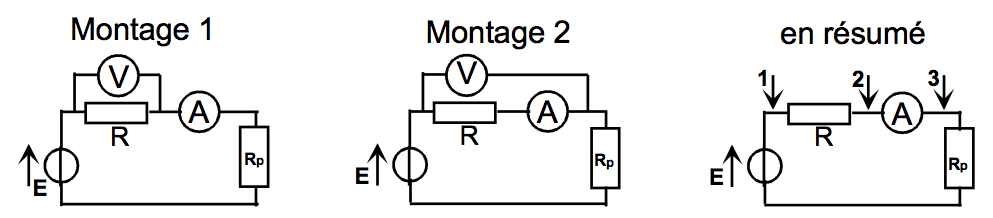
\includegraphics[width=\linewidth]{TP01_schema}
\end{center}

\subsection{Observations}

Voici comment présenter un tableau de résultats:

$$
% Tableau en mode math (en mode texte, il faut utiliser un {tabular})
\begin{array}{c|c|c} % Les barres donnent les barres verticales, les "c" pour "centrage" 
	&	\text{Exp 1}	&	\text{Exp 2}	% Les bords des cellules sont délimitées par des &
    \\ \hline\hline % Passage à la ligne et ligne horizontale double
U\U{(V)}	&	\numprint{12,3}	&	\numprint{10,2}	\\
I\U{(mA)}	&	\numprint{1,23}	&	\numprint{1,54}	\\
\end{array}
$$

% On peut introduire du code Python pour faire les calculs difficiles
\begin{pycode}
U  = 12.345
DU = 0.2/100*U + 5*0.001
I  = 1.321e-3
DI = 1/100*I + 6*0.001e-3
R  = U/I
DR = R*((DU/U)**2+(DI/I)**2)**0.5
\end{pycode}

% et utiliser les quantités calculées via la commande \py{}
On trouve $U=\py{round(U,2)}\pm\py{round(DU,2)}\U{V}$ et $I=\py{round(I*1e3,2)}\pm\py{round(DI*1e3,2)}\U{mA}$. Comme $R=U/I$, la formule de propagation des incertitudes composées lors d'une division donne

$$\Delta R = R\times\sqrt{\left(\frac{\Delta U}{U}\right)^{\!2} + \left(\frac{\Delta I}{I}\right)^{\!2}} = \py{round(DR/1e3,2)}\U{k\Omega}$$

\noindent
soit finalement

$$\boxed{R = \py{round(R/1e3,2)}\pm\py{round(DR/1e3,2)}\U{k\Omega}}$$


% On peut aussi demander d'afficher le code python en plus de l'exécuter
\begin{code}
\begin{pyblock}[][numbers=left]
U  = 12.345
DU = 0.2/100*U + 5*0.001
I  = 1.321e-3
DI = 1/100*I + 6*0.001e-3
R  = U/I
DR = R*((DU/U)**2+(DI/I)**2)**0.5
\end{pyblock}
\end{code}

\subsection{Conclusion}

\section{Seconde partie}

\subsection{Expérience}

\subsection{Observations}

\subsection{Conclusion}

\section{Conclusion générale du TP}

\end{document}